
% !TeX spellcheck = en

\chapter{Introduction to Liquibase}
\section{Overview}
\marginpar{Overview \cite{Liquibase}}%
The Liquibase tool is a database schema change management solution that enables fast and safe database change releases from development to production. Liquibase \cite{Liquibase} will help to:

\begin{itemize}
	\item Control database schema changes for specific versions.
	\item Eliminate errors and delays when releasing databases.
	\item Automatically order scripts for deployment.
	\item Easily rollback changes.
	\item Collaborate with already used tools.
\end{itemize}

\marginpar{Support \cite{Liquibase}}%
Additionally, Liquibase works with over 50 databases categorized on different verification levels. Table \ref{tab:IntroductionToLiquibase:DBVerificationLevels}

\begin{table}[H]
	\centering
	\ra{1.3}
	\begin{tabularx}{\textwidth}{ll} 
		\toprule
		Verification Level & Description \\ 
		\midrule
		Guaranteed & \makecell[l]{Database tested and certified by Liquibase and works with all\\ Liquibase Pro capabilities.} \\[10pt]
		Foundational & \makecell[l]{Database tested and certified by Liquibase with the full set of\\ open source capabilities. Liquibase Pro functionality is not\\ guaranteed.} \\[15pt]
		Compatible & \makecell[l]{Widely reported as working by the community but has incomplete\\ functionality. Best effort support provided by Liquibase.} \\[10pt]
		Unverified & \makecell[l]{Not enough information for assessment. Best effort support\\ provided through community forums.} \\
		\bottomrule
	\end{tabularx}
	\caption{Supported Database, Verification Levels}
	\label{tab:IntroductionToLiquibase:DBVerificationLevels}
\end{table}

\marginpar{Pricing and Editions \cite{Liquibase}}%
Liquibase \cite{Liquibase} comes in three editions with different pricing: Free, Pro and Enterprise. Each edition adds more functionality than the preceding. However, the free, open-source version provides all the core functionalities needed. The Pro and Enterprise version targets larger teams with ten or more members. 

\marginpar{Community}%
Stars on GitHub: 3'600 (27. December 2022)\\
Tags on StackOverflow: 3,530 (27. December 2022)\\

\section{Functionality}
\marginpar{Organisation \cite{Liquibase}}%
Liquibase uses a changelog file to list database changes sequentially. Each change is defined in the changeset format and contains change types, which specify the operations to apply.

\begin{figure}[H]
	\centering
	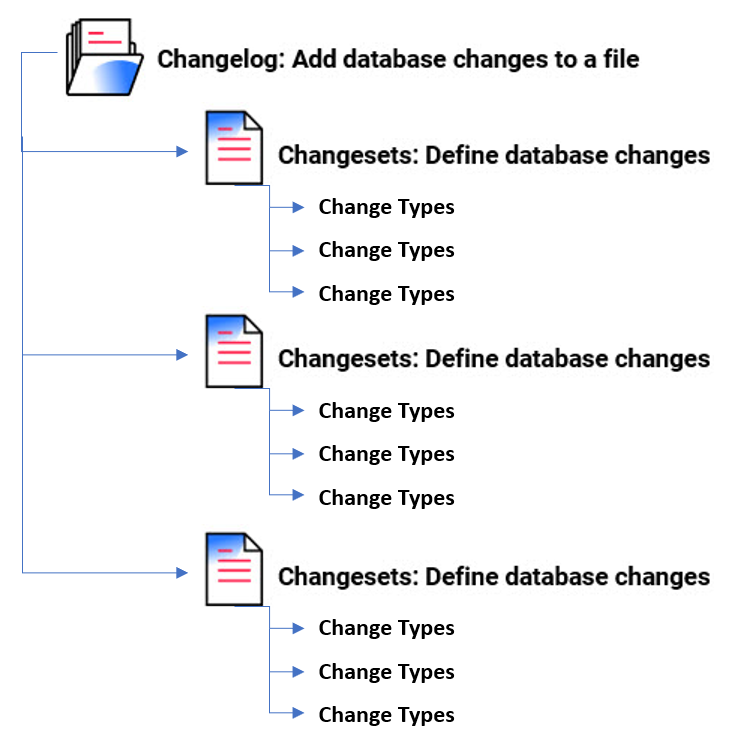
\includegraphics[width=0.65\textwidth]{./chapters/intro_liquibase/images/changelog-structure.png}
	\caption[Liquibase Organisation - Source: \cite{Liquibase}]{Liquibase Organisation}
	\label{fig:IntroductionToLiquibase:LiquibaseChangelogStructure}
\end{figure}


\section{Main Commands}



\section{Installation and Setup}
\todo{updateSQL}
Die Funktion updateSQL von LiquiBase
Ermöglicht, die anstehende Migration zunächst als SQL-Befehle auszugeben, z.B. zu Review- Zwecken.
Ist bei Flyway nicht relevant, da Plain-SQL-Skripte verwendet werden


\newpage